\section{Incremental Synchronization of Shapes}
\label{sec:prism}

The cornerstone artifact defining a DSL in any LV is its abstract syntax.
The way abstract syntax is expressed differs drastically from one LV to another: GEMOC~\cite{bousse2016execution} and Xtext~\cite{bettini2016implementing}---under the hood---use Ecore metamodels~\cite{steinberg2008emf}; MPS~\cite{voelter2014generic} uses \emph{concepts}; Rascal~\cite{klint2010easy} uses Algebraic Data Types (ADT); \etc.
Language embedding techniques, on the other hand, use the constructs of an host language to materialize the abstractions of a DSL in the host language itself (\eg~a set of Java classes).
Concrete models are then built as instances of the corresponding abstract syntax formalism:~Ecore models, ADT values, Java ASTs, \etc.
The tools defined within a particular LV (an interpreter in Rascal, an editor in EMF) manipulate models in the corresponding formalism (respectively, ADT values and Ecore models).
These formalisms radically differ in many ways:~object-oriented vs. functional, graphs vs. trees, mutable ASG vs. immutable ASTs, cross-references vs. symbolic names, \etc.
However, it is neither possible nor desirable to establish a common formalism upon which all LVs would agree:~mapping those is out of reach.

\Cref{fig:concepts} gives an overview of the concepts we use throughout this paper.
A ``conceptual'' language $\mathcal{L}$ is materialized as a shape $\mathcal{S}$ in a LV.
$\mathcal{S}$ can therefore be seen as the implementation of $\mathcal{L}$ in the LV.
Similarly, a ``conceptual'' model $m$ conforming to $\mathcal{L}$ is materialized as an incarnation $\mathcal{I}$ conforming to the shape $\mathcal{S}$ in a LV.
\td{Not very proud of the ``conceptual''. Any idea?}
As each shape manipulate models in its own formalism, the various incarnations $I$ of the same model $m$ must remain synchronized with each others.

A naive way to bridge different LVs would be to define bidirectional transformations between the abstract syntax formalisms of every pair $\langle LV, LV' \rangle$.
Doing so however would close the world around the chosen set of LVs.
As every LV holds particular extra information on its incarnations, such as layout in an editor, runtime data for running models, or context information around API calls, the synchronization must be incremental.

In our approach, \prism, every change occuring on one incarnation is shipped to all other incarnations of the same model.
Every shape is responsible for\dots

\begin{figure}[bt]
	\centering
	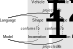
\includegraphics[width=.8\columnwidth]{figures/concepts}
	\caption{Languages (resp.~models) are projected as shapes (resp.~incarnations) in LVs. Just as models conform to languages, incarnations conform to shapes.\\NB: \emph{projectedAs $\Rightarrow$ realizedBy / materializedBy}?}
	\label{fig:concepts}
\end{figure}

\begin{enumerate}
	\item Synchronize the various in-memory representations of the same model;
	\item Allow every LV to maintain the extra information it needs to properly work (layout information in graphical and textual editors, runtime state, AST context, \etc);
	\item From 1. and 2., it follows that the synchronization must be incremental.
\end{enumerate}

\subsection{Projection of language}
In \Cref{fig:concepts} we describe a projection of language and model in different LVs.
A model is projected into several LVs.
The projection takes the form of incarnations the same model in the different LVs.
We define the projection of model as following:
\begin{definition}
A projection of model is a relation between a conceptual model and its different incarnations in the LVs.
All of theses incarnations represent the same model but in different formalisms and technologies.
Incarnations have to be synchronized, i.e., any change on an incarnation is a change on the conceptual model and thus other incarnations have to apply the same change.
\end{definition}
In a similar way the language is projected as shapes into the LVs.
We define a shape as following:
\begin{definition}
A shape is a projection of a language in a particular LV.
It is equivalent to a language implementation in this LV.
Therefore if a model is conform to the language, all its incarnations in this LV are conform to the shape.
\end{definition}
Mirroring model and language, each incarnation of a LVs is conform to a shape.

Since the LVs are isolated but incarnations represent the same model, there is a need for a synchronization mechanism.


%\begin{definition}
%A prism in the context of a model projection is the mechanism that allows the different incarnations of the model to be in equivalent state and to synchronize.
%\end{definition}

\subsection{Synchronization of incarnations}

\begin{figure}[bt]
	\centering
	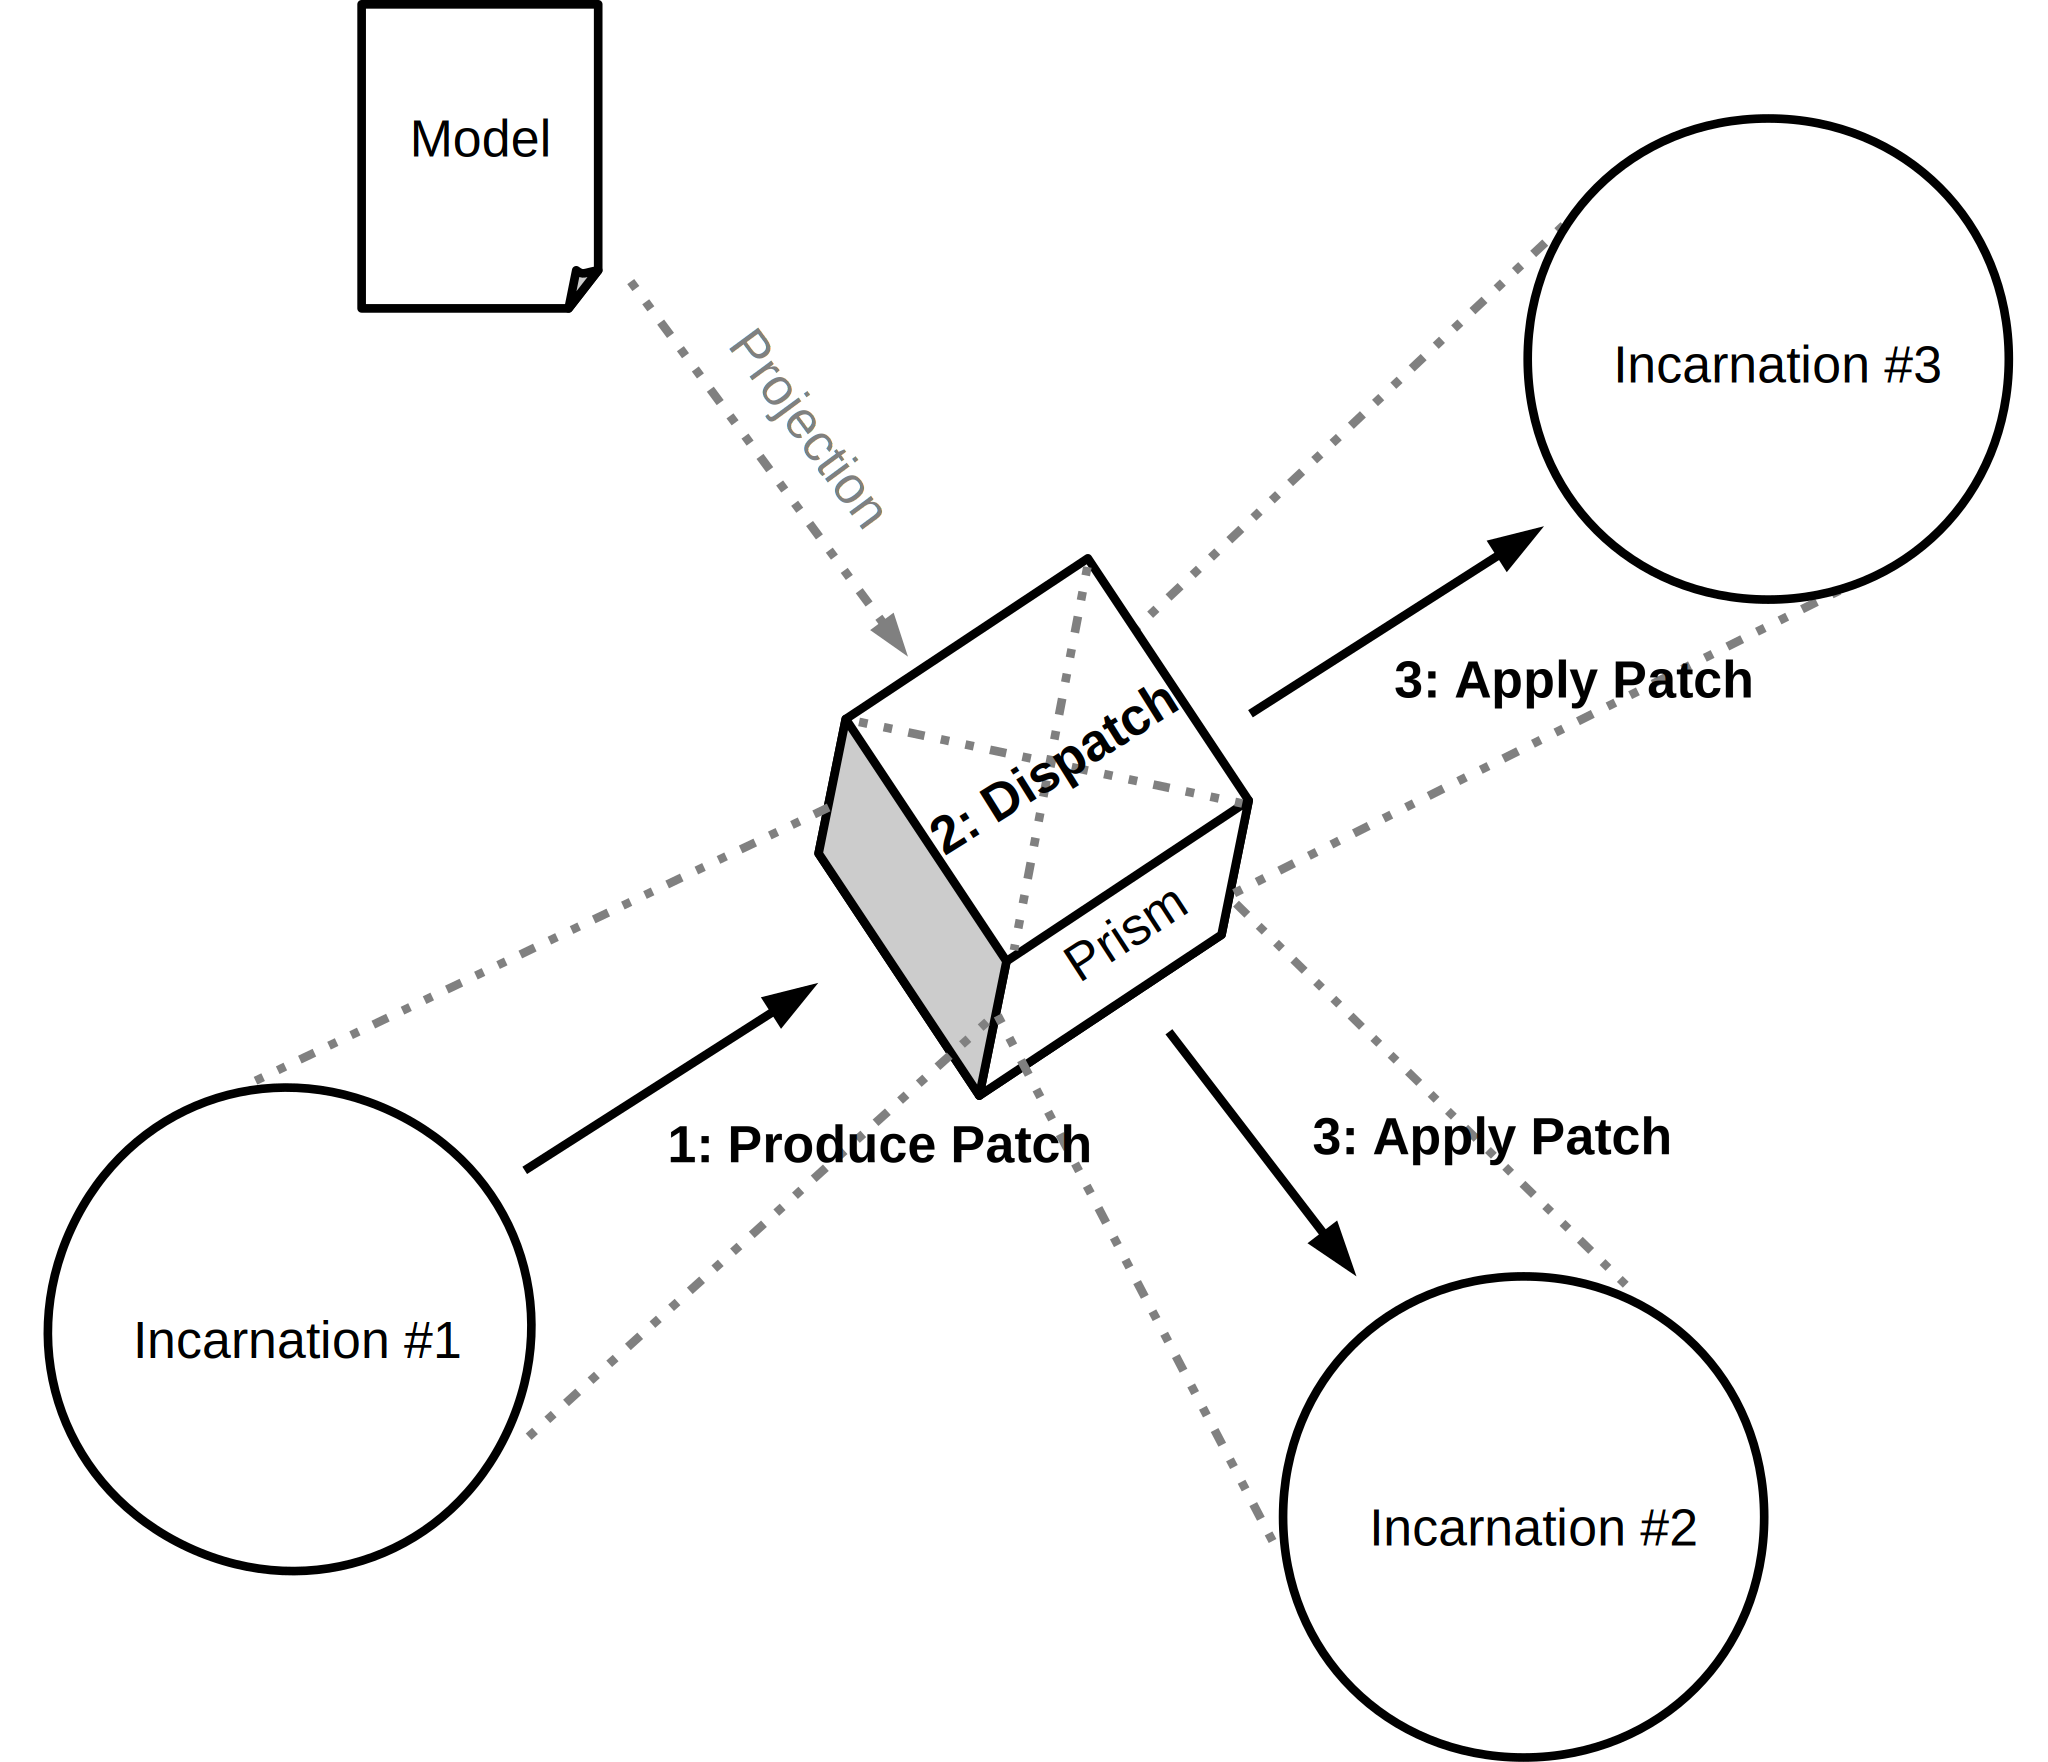
\includegraphics[width=.6\columnwidth]{figures/prism}
	\caption{A model projected in different LVs}
	\label{fig:prism}
\end{figure}

The key underlying idea of our approach is to provide the capability, at any time, to ``project'' a given model in any of its shapes and to synchronize those shapes whenever one of them is updated.
We enable the projection of a given model as an ADT value, to be manipulated in the Rascal TS, or as an Ecore model, to be manipulated in the EMF TS.

Instead, our approach keeps the TS fully independent and builds a communication bus between them.
Both representations of the same model in various TS are kept in memory to allow online synchronization of the same models manipulated by different stakeholders in different shapes.
When a changes occurs on either side, this side is responsible for generating a \emph{patch} (aka. \de or edit script~\cite{rozen2017towards}), that stores the changes on the model that have been realized on this side.
The communication bus then ships this patch to all the other sides.
Every side interprets the patch in its own way to keep the representation synchronized.
On the EMF side, for instance, the patch is interpreted as a set of changes that impact an Ecore model, while on the Rascal side it is interpreted as a set of changes that impact a value conforming to the ADT defining the AS of the language.

It is important to note that each TS may want to preserve certain information across the patches that are specific to the TS.
A textual editor in Rascal, for instance, needs to keep some of the parsing information to maintain layout whenever patches are applied.
So it should be possible to apply the patch while maintaining the extra information specific to a given TS.

Automatically generating language implementations in different TS is beyond the scope of this paper.\footnote{Indeed, this would actually require to build some kind of BX between all AS formalisms; so, nope!} Instead, given various shapes of a language, implemented by hand, we provide the means to automatically synchronize the projections of a model.

\begin{lstlisting}[label=lst:delta-adt, caption={CRUD-like \ds structure definition in Rascal}, language=Rascal]
@doc{A patch consists of a sequence of edits}
alias Patch = tuple[Id root, Edits edits];

@doc{Edits are operations attached to object identities}
alias Edits = lrel[Id obj, Edit edit];

data Edit
  = put(str field, value val)
  | unset(str field)
  | ins(str field, int pos, value val)
  | del(str field, int pos)
  | create(str class) 
  | destroy();
\end{lstlisting}

It is important to note that ``projections'' have no relation whatsoever with projectional editing.
A projection denotes the incarnation of a model in a particular shape of a language.
In \Cref{fig:motivating-fsm}, the lower part depicts three projections of the same \texttt{Button} state machine model in three shapes of the FSM language.
We use the term ``language'' to refer to the specification of a language independently from its realization in a given TS.
A concrete implementation of a language is a ``shape''.
An instance of a shape, \ie~a particular model in a particular TS, is a ``projection'' of a ``virtual'' model.
Metamorphic synchronization refers to the ability to synchronize the projections of a given model for every shapes of a language.



